\chapter{Additional Experimental Results}
\vspace{-2em}
\section{Results from \chapref{ch:m3}}
\vspace{-2em}

\setlength\figureheight{0.37\textwidth}
\setlength\figurewidth{0.55\textwidth}
\renewcommand{\subflen}{1.0\textwidth}
\begin{figure}[h!]
  \captionsetup[subfigure]{oneside,margin={2em,0em}}
  \begin{subfigure}[b]{\subflen}
    \centering
    \begin{tikzpicture}


\begin{axis}[%
tick label style={/pgf/number format/fixed,font=\sffamily\small},
label style={font=\sffamily\small},
legend style={font=\sffamily\small},
view={0}{90},
width=\figurewidth,
height=\figureheight,
xmin=0, xmax=200,
xtick={0, 100, 200},
xticklabels={0, 100, 200},
scaled x ticks=false,
xlabel={Time (ms)},
xlabel shift=0em,
ymin=1, ymax=1.52,
ytick={1, 1.5},
yticklabels={1, 1.5},
ylabel={PSRF},
ylabel shift=-1em,
major tick length=2pt,
axis lines*=left,
legend cell align=left,
clip marker paths=true,
legend style={anchor=north east,at={(1,1)},draw=none,row sep=0em},
every axis plot/.append style={
  line width=1.5pt,
  opacity=0.8,
}
]

\addplot [
color=col1dark,
densely dashed,
]
coordinates{
(8.110889,3.597939) +- (-0.282843,0.282843)(9.124750,3.040631) +- (-0.197440,0.197440)(10.138612,2.691309) +- (-0.160233,0.160233)(11.152473,2.554452) +- (-0.165238,0.165238)(12.166334,2.413226) +- (-0.160241,0.160241)(13.180195,2.330296) +- (-0.148466,0.148466)(14.194056,2.215460) +- (-0.130796,0.130796)(15.207917,2.169512) +- (-0.130263,0.130263)(16.221778,2.082272) +- (-0.130343,0.130343)(17.235640,2.028475) +- (-0.144012,0.144012)(18.249501,2.014070) +- (-0.189635,0.189635)(19.263362,2.059465) +- (-0.282843,0.282843)(20.277223,1.948577) +- (-0.207447,0.207447)(21.291084,1.888214) +- (-0.187895,0.187895)(22.304945,1.800753) +- (-0.146235,0.146235)(23.318807,1.749965) +- (-0.125414,0.125414)(24.332668,1.717381) +- (-0.149604,0.149604)(25.346529,1.704961) +- (-0.179373,0.179373)(26.360390,1.685182) +- (-0.188536,0.188536)(27.374251,1.651440) +- (-0.194696,0.194696)(28.388112,1.565033) +- (-0.110935,0.110935)(29.401973,1.494971) +- (-0.060617,0.060617)(30.415835,1.448536) +- (-0.037580,0.037580)(31.429696,1.423904) +- (-0.030389,0.030389)(32.443557,1.404557) +- (-0.025724,0.025724)(33.457418,1.388615) +- (-0.024165,0.024165)(34.471279,1.375496) +- (-0.022723,0.022723)(35.485140,1.365812) +- (-0.022431,0.022431)(36.499002,1.359307) +- (-0.022667,0.022667)(37.512863,1.357107) +- (-0.023374,0.023374)(38.526724,1.353670) +- (-0.024974,0.024974)(39.540585,1.349603) +- (-0.026614,0.026614)(40.554446,1.341914) +- (-0.026115,0.026115)(40.554446,1.341914) +- (-0.026115,0.026115)(42.582168,1.327010) +- (-0.025499,0.025499)(44.609891,1.309038) +- (-0.022776,0.022776)(46.637613,1.291903) +- (-0.021510,0.021510)(48.665335,1.276404) +- (-0.019627,0.019627)(50.693058,1.265232) +- (-0.019791,0.019791)(52.720780,1.257915) +- (-0.022160,0.022160)(54.748502,1.245602) +- (-0.022382,0.022382)(56.776225,1.229363) +- (-0.019007,0.019007)(58.803947,1.212160) +- (-0.014853,0.014853)(60.831669,1.202877) +- (-0.014921,0.014921)(62.859391,1.194305) +- (-0.016019,0.016019)(64.887114,1.187061) +- (-0.016566,0.016566)(66.914836,1.181264) +- (-0.015779,0.015779)(68.942558,1.176979) +- (-0.015684,0.015684)(70.970281,1.173301) +- (-0.016778,0.016778)(72.998003,1.166561) +- (-0.015625,0.015625)(75.025725,1.160849) +- (-0.014327,0.014327)(77.053448,1.157492) +- (-0.013240,0.013240)(79.081170,1.152301) +- (-0.012648,0.012648)(81.108892,1.146251) +- (-0.010389,0.010389)(83.136615,1.142146) +- (-0.008755,0.008755)(85.164337,1.138389) +- (-0.008279,0.008279)(87.192059,1.134830) +- (-0.007781,0.007781)(89.219781,1.131334) +- (-0.007385,0.007385)(91.247504,1.129364) +- (-0.007120,0.007120)(93.275226,1.127263) +- (-0.007972,0.007972)(95.302948,1.124395) +- (-0.008520,0.008520)(97.330671,1.119219) +- (-0.008856,0.008856)(99.358393,1.117366) +- (-0.010033,0.010033)(101.386115,1.114105) +- (-0.008819,0.008819)(103.413838,1.113725) +- (-0.008468,0.008468)(105.441560,1.111648) +- (-0.008166,0.008166)(107.469282,1.109619) +- (-0.007836,0.007836)(109.497005,1.107001) +- (-0.007309,0.007309)(111.524727,1.104818) +- (-0.006968,0.006968)(113.552449,1.104075) +- (-0.006324,0.006324)(115.580171,1.102976) +- (-0.006398,0.006398)(117.607894,1.100722) +- (-0.006288,0.006288)(119.635616,1.097873) +- (-0.005578,0.005578)(121.663338,1.095111) +- (-0.005033,0.005033)(123.691061,1.093478) +- (-0.005158,0.005158)(125.718783,1.091610) +- (-0.005177,0.005177)(127.746505,1.090405) +- (-0.005001,0.005001)(129.774228,1.089527) +- (-0.004982,0.004982)(131.801950,1.088855) +- (-0.004821,0.004821)(133.829672,1.087810) +- (-0.004819,0.004819)(135.857395,1.086178) +- (-0.004890,0.004890)(137.885117,1.083872) +- (-0.004823,0.004823)(139.912839,1.082651) +- (-0.004757,0.004757)(141.940561,1.082000) +- (-0.004411,0.004411)(143.968284,1.081654) +- (-0.004404,0.004404)(145.996006,1.080664) +- (-0.004261,0.004261)(148.023728,1.079681) +- (-0.004000,0.004000)(150.051451,1.078145) +- (-0.004157,0.004157)(152.079173,1.077135) +- (-0.004285,0.004285)(154.106895,1.076356) +- (-0.004383,0.004383)(156.134618,1.075704) +- (-0.004286,0.004286)(158.162340,1.074393) +- (-0.004038,0.004038)(160.190062,1.072686) +- (-0.003808,0.003808)(162.217785,1.071898) +- (-0.003671,0.003671)(164.245507,1.070577) +- (-0.003569,0.003569)(166.273229,1.068997) +- (-0.003373,0.003373)(168.300951,1.067786) +- (-0.003359,0.003359)(170.328674,1.067305) +- (-0.003437,0.003437)(172.356396,1.066197) +- (-0.003413,0.003413)(174.384118,1.064406) +- (-0.003289,0.003289)(176.411841,1.062878) +- (-0.003119,0.003119)(178.439563,1.061796) +- (-0.003118,0.003118)(180.467285,1.061438) +- (-0.003328,0.003328)(182.495008,1.061019) +- (-0.003352,0.003352)(184.522730,1.060327) +- (-0.003275,0.003275)(186.550452,1.059904) +- (-0.003248,0.003248)(188.578174,1.059435) +- (-0.003126,0.003126)(190.605897,1.058691) +- (-0.002941,0.002941)(192.633619,1.057888) +- (-0.002763,0.002763)(194.661341,1.057200) +- (-0.002759,0.002759)(196.689064,1.056826) +- (-0.002693,0.002693)(198.716786,1.056174) +- (-0.002721,0.002721)(200.744508,1.055308) +- (-0.002654,0.002654)(202.772231,1.054398) +- (-0.002602,0.002602)
};
\addlegendentry{\textsc{Gibbs}}


\addplot [
color=col2
]
coordinates{
(4.691006,2.314380) +- (-0.145936,0.145936)(5.863757,2.004462) +- (-0.127423,0.127423)(7.036509,1.793518) +- (-0.080239,0.080239)(8.209260,1.631944) +- (-0.067338,0.067338)(9.382012,1.547655) +- (-0.050816,0.050816)(10.554763,1.467467) +- (-0.045281,0.045281)(11.727515,1.434199) +- (-0.047724,0.047724)(12.900266,1.387869) +- (-0.026698,0.026698)(14.073018,1.352802) +- (-0.024894,0.024894)(15.245769,1.325987) +- (-0.022519,0.022519)(16.418521,1.300620) +- (-0.018924,0.018924)(17.591272,1.276801) +- (-0.015945,0.015945)(18.764024,1.258876) +- (-0.015658,0.015658)(19.936775,1.247336) +- (-0.015910,0.015910)(21.109527,1.231760) +- (-0.014686,0.014686)(22.282278,1.220108) +- (-0.014804,0.014804)(23.455030,1.209891) +- (-0.016687,0.016687)(24.627781,1.197965) +- (-0.017494,0.017494)(25.800533,1.187772) +- (-0.017134,0.017134)(26.973284,1.181613) +- (-0.016117,0.016117)(28.146036,1.175375) +- (-0.015438,0.015438)(29.318787,1.167047) +- (-0.014963,0.014963)(30.491539,1.162951) +- (-0.014282,0.014282)(31.664290,1.159416) +- (-0.013639,0.013639)(32.837042,1.151083) +- (-0.012802,0.012802)(34.009793,1.143855) +- (-0.013366,0.013366)(35.182545,1.139644) +- (-0.013836,0.013836)(36.355296,1.136401) +- (-0.012880,0.012880)(37.528048,1.130305) +- (-0.011110,0.011110)(38.700799,1.127232) +- (-0.010790,0.010790)(39.873550,1.121431) +- (-0.010224,0.010224)(41.046302,1.116844) +- (-0.009764,0.009764)(42.219053,1.113843) +- (-0.009180,0.009180)(43.391805,1.109543) +- (-0.008657,0.008657)(44.564556,1.105246) +- (-0.008078,0.008078)(45.737308,1.101941) +- (-0.007431,0.007431)(46.910059,1.097746) +- (-0.006427,0.006427)(46.910059,1.097746) +- (-0.006427,0.006427)(49.255562,1.090858) +- (-0.005703,0.005703)(51.601065,1.085136) +- (-0.004712,0.004712)(53.946568,1.082785) +- (-0.004480,0.004480)(56.292071,1.078993) +- (-0.004481,0.004481)(58.637574,1.075416) +- (-0.004278,0.004278)(60.983077,1.072572) +- (-0.004408,0.004408)(63.328580,1.072164) +- (-0.004253,0.004253)(65.674083,1.071047) +- (-0.003945,0.003945)(68.019586,1.068267) +- (-0.003995,0.003995)(70.365089,1.064680) +- (-0.003782,0.003782)(72.710592,1.062878) +- (-0.003607,0.003607)(75.056095,1.060127) +- (-0.002978,0.002978)(77.401598,1.057291) +- (-0.002852,0.002852)(79.747101,1.056389) +- (-0.002972,0.002972)(82.092604,1.054495) +- (-0.002850,0.002850)(84.438107,1.052421) +- (-0.002805,0.002805)(86.783610,1.052303) +- (-0.003047,0.003047)(89.129113,1.051432) +- (-0.002882,0.002882)(91.474616,1.049071) +- (-0.002860,0.002860)(93.820119,1.048121) +- (-0.002986,0.002986)(96.165622,1.046968) +- (-0.002974,0.002974)(98.511125,1.046242) +- (-0.002929,0.002929)(100.856628,1.046152) +- (-0.002783,0.002783)(103.202131,1.045838) +- (-0.002628,0.002628)(105.547634,1.044434) +- (-0.002501,0.002501)(107.893137,1.043060) +- (-0.002611,0.002611)(110.238640,1.042289) +- (-0.002473,0.002473)(112.584143,1.041161) +- (-0.002194,0.002194)(114.929646,1.040078) +- (-0.002039,0.002039)(117.275149,1.038894) +- (-0.001963,0.001963)(119.620651,1.037761) +- (-0.002019,0.002019)(121.966154,1.036455) +- (-0.001902,0.001902)(124.311657,1.035295) +- (-0.001652,0.001652)(126.657160,1.034810) +- (-0.001550,0.001550)(129.002663,1.034331) +- (-0.001533,0.001533)(131.348166,1.033830) +- (-0.001393,0.001393)(133.693669,1.032976) +- (-0.001362,0.001362)(136.039172,1.032553) +- (-0.001368,0.001368)(138.384675,1.031991) +- (-0.001444,0.001444)(140.730178,1.031694) +- (-0.001432,0.001432)(143.075681,1.031078) +- (-0.001410,0.001410)(145.421184,1.030946) +- (-0.001536,0.001536)(147.766687,1.030691) +- (-0.001492,0.001492)(150.112190,1.030606) +- (-0.001415,0.001415)(152.457693,1.030274) +- (-0.001521,0.001521)(154.803196,1.029901) +- (-0.001567,0.001567)(157.148699,1.029501) +- (-0.001596,0.001596)(159.494202,1.029197) +- (-0.001490,0.001490)(161.839705,1.028674) +- (-0.001432,0.001432)(164.185208,1.028292) +- (-0.001420,0.001420)(166.530711,1.027638) +- (-0.001465,0.001465)(168.876214,1.027133) +- (-0.001453,0.001453)(171.221717,1.027022) +- (-0.001433,0.001433)(173.567220,1.026421) +- (-0.001474,0.001474)(175.912723,1.025866) +- (-0.001395,0.001395)(178.258226,1.025313) +- (-0.001397,0.001397)(180.603729,1.025126) +- (-0.001384,0.001384)(182.949232,1.024998) +- (-0.001477,0.001477)(185.294735,1.024660) +- (-0.001446,0.001446)(187.640238,1.024171) +- (-0.001362,0.001362)(189.985741,1.023864) +- (-0.001253,0.001253)(192.331244,1.023532) +- (-0.001167,0.001167)(194.676747,1.023254) +- (-0.001154,0.001154)(197.022249,1.023072) +- (-0.001145,0.001145)(199.367752,1.022695) +- (-0.001132,0.001132)(201.713255,1.022507) +- (-0.001124,0.001124)(204.058758,1.022286) +- (-0.001143,0.001143)(206.404261,1.021894) +- (-0.001132,0.001132)(208.749764,1.021687) +- (-0.001104,0.001104)(211.095267,1.021078) +- (-0.000988,0.000988)(213.440770,1.020705) +- (-0.000968,0.000968)(215.786273,1.020400) +- (-0.000900,0.000900)(218.131776,1.020334) +- (-0.000907,0.000907)(220.477279,1.020393) +- (-0.000906,0.000906)(222.822782,1.020249) +- (-0.000837,0.000837)(225.168285,1.020091) +- (-0.000844,0.000844)(227.513788,1.019827) +- (-0.000798,0.000798)(229.859291,1.019461) +- (-0.000836,0.000836)(232.204794,1.019257) +- (-0.000829,0.000829)(234.550297,1.019229) +- (-0.000875,0.000875)
};
\addlegendentry{\textsc{Combo-R}}


\addplot [
color=col3
]
coordinates{
(2.353020,3.854406) +- (-0.282843,0.282843)(3.529530,2.516837) +- (-0.198273,0.198273)(4.706040,2.080291) +- (-0.204548,0.204548)(5.882550,1.761562) +- (-0.101370,0.101370)(7.059060,1.588895) +- (-0.068315,0.068315)(8.235570,1.530598) +- (-0.077335,0.077335)(9.412080,1.472095) +- (-0.088279,0.088279)(10.588590,1.407313) +- (-0.069317,0.069317)(11.765099,1.328349) +- (-0.050041,0.050041)(12.941609,1.280189) +- (-0.046740,0.046740)(14.118119,1.241093) +- (-0.028634,0.028634)(15.294629,1.225659) +- (-0.018168,0.018168)(16.471139,1.214143) +- (-0.016083,0.016083)(17.647649,1.199464) +- (-0.015557,0.015557)(18.824159,1.192993) +- (-0.017602,0.017602)(20.000669,1.182354) +- (-0.016598,0.016598)(21.177179,1.173964) +- (-0.016687,0.016687)(22.353689,1.162564) +- (-0.013994,0.013994)(23.530199,1.153207) +- (-0.012485,0.012485)(24.706709,1.146027) +- (-0.011376,0.011376)(25.883219,1.138410) +- (-0.011042,0.011042)(27.059729,1.132240) +- (-0.010125,0.010125)(28.236239,1.124508) +- (-0.009295,0.009295)(29.412749,1.120885) +- (-0.010133,0.010133)(30.589259,1.114675) +- (-0.009175,0.009175)(31.765769,1.110488) +- (-0.008958,0.008958)(32.942279,1.106881) +- (-0.007907,0.007907)(34.118789,1.104418) +- (-0.007560,0.007560)(35.295298,1.099178) +- (-0.007433,0.007433)(36.471808,1.094869) +- (-0.007824,0.007824)(37.648318,1.092353) +- (-0.007203,0.007203)(38.824828,1.089835) +- (-0.006443,0.006443)(40.001338,1.086294) +- (-0.005841,0.005841)(41.177848,1.083016) +- (-0.004871,0.004871)(42.354358,1.080625) +- (-0.004230,0.004230)(43.530868,1.078600) +- (-0.003971,0.003971)(44.707378,1.075129) +- (-0.003631,0.003631)(45.883888,1.073524) +- (-0.003559,0.003559)(47.060398,1.071891) +- (-0.003385,0.003385)(47.060398,1.071891) +- (-0.003385,0.003385)(49.413418,1.066995) +- (-0.003261,0.003261)(51.766438,1.064854) +- (-0.003031,0.003031)(54.119458,1.062135) +- (-0.003158,0.003158)(56.472478,1.060072) +- (-0.002924,0.002924)(58.825497,1.058380) +- (-0.002652,0.002652)(61.178517,1.055289) +- (-0.003135,0.003135)(63.531537,1.053504) +- (-0.002473,0.002473)(65.884557,1.051133) +- (-0.002215,0.002215)(68.237577,1.049357) +- (-0.002129,0.002129)(70.590597,1.048042) +- (-0.002443,0.002443)(72.943617,1.046165) +- (-0.002292,0.002292)(75.296637,1.044985) +- (-0.002335,0.002335)(77.649657,1.043813) +- (-0.002302,0.002302)(80.002677,1.042142) +- (-0.002126,0.002126)(82.355696,1.040972) +- (-0.001732,0.001732)(84.708716,1.038792) +- (-0.001605,0.001605)(87.061736,1.037901) +- (-0.001482,0.001482)(89.414756,1.037031) +- (-0.001745,0.001745)(91.767776,1.036926) +- (-0.002238,0.002238)(94.120796,1.036016) +- (-0.002091,0.002091)(96.473816,1.034859) +- (-0.002239,0.002239)(98.826836,1.033716) +- (-0.002164,0.002164)(101.179856,1.032822) +- (-0.001992,0.001992)(103.532876,1.031838) +- (-0.001809,0.001809)(105.885895,1.030816) +- (-0.001774,0.001774)(108.238915,1.030378) +- (-0.001692,0.001692)(110.591935,1.030052) +- (-0.001777,0.001777)(112.944955,1.029630) +- (-0.001723,0.001723)(115.297975,1.028859) +- (-0.001648,0.001648)(117.650995,1.028342) +- (-0.001664,0.001664)(120.004015,1.027460) +- (-0.001711,0.001711)(122.357035,1.026793) +- (-0.001637,0.001637)(124.710055,1.026026) +- (-0.001552,0.001552)(127.063074,1.025250) +- (-0.001265,0.001265)(129.416094,1.025001) +- (-0.001289,0.001289)(131.769114,1.024221) +- (-0.001330,0.001330)(134.122134,1.023217) +- (-0.001235,0.001235)(136.475154,1.023087) +- (-0.001262,0.001262)(138.828174,1.022697) +- (-0.001187,0.001187)(141.181194,1.022573) +- (-0.001180,0.001180)(143.534214,1.022419) +- (-0.001269,0.001269)(145.887234,1.022147) +- (-0.001212,0.001212)(148.240254,1.021630) +- (-0.001206,0.001206)(150.593273,1.021636) +- (-0.001243,0.001243)(152.946293,1.021386) +- (-0.001207,0.001207)(155.299313,1.021237) +- (-0.001212,0.001212)(157.652333,1.020897) +- (-0.001196,0.001196)(160.005353,1.020573) +- (-0.001154,0.001154)(162.358373,1.020276) +- (-0.001089,0.001089)(164.711393,1.019911) +- (-0.001184,0.001184)(167.064413,1.019570) +- (-0.001224,0.001224)(169.417433,1.019220) +- (-0.001139,0.001139)(171.770453,1.018847) +- (-0.001054,0.001054)(174.123472,1.018390) +- (-0.000911,0.000911)(176.476492,1.018087) +- (-0.000910,0.000910)(178.829512,1.018215) +- (-0.001009,0.001009)(181.182532,1.017975) +- (-0.000981,0.000981)(183.535552,1.017773) +- (-0.000918,0.000918)(185.888572,1.017623) +- (-0.000880,0.000880)(188.241592,1.017201) +- (-0.000808,0.000808)(190.594612,1.017108) +- (-0.000833,0.000833)(192.947632,1.016947) +- (-0.000744,0.000744)(195.300652,1.016976) +- (-0.000757,0.000757)(197.653671,1.016918) +- (-0.000846,0.000846)(200.006691,1.016655) +- (-0.000857,0.000857)(202.359711,1.016267) +- (-0.000828,0.000828)(204.712731,1.016105) +- (-0.000774,0.000774)(207.065751,1.015787) +- (-0.000799,0.000799)(209.418771,1.015690) +- (-0.000837,0.000837)(211.771791,1.015584) +- (-0.000785,0.000785)(214.124811,1.015477) +- (-0.000837,0.000837)(216.477831,1.015410) +- (-0.000880,0.000880)(218.830851,1.015213) +- (-0.000865,0.000865)(221.183870,1.014935) +- (-0.000832,0.000832)(223.536890,1.014694) +- (-0.000838,0.000838)(225.889910,1.014629) +- (-0.000778,0.000778)(228.242930,1.014533) +- (-0.000751,0.000751)(230.595950,1.014393) +- (-0.000742,0.000742)(232.948970,1.014260) +- (-0.000782,0.000782)(235.301990,1.014056) +- (-0.000720,0.000720)
};
\addlegendentry{\textsc{Combo-I}}

\end{axis}
\end{tikzpicture}

    \vspace{-0.5em}
    \caption{\textsc{Water}}
    \label{fig:water1_time}
  \end{subfigure}\\
  \begin{subfigure}[b]{\subflen}
    \centering
    \begin{tikzpicture}


\begin{axis}[%
tick label style={/pgf/number format/fixed,font=\sffamily\small},
label style={font=\sffamily\small},
legend style={font=\sffamily\small},
view={0}{90},
width=\figurewidth,
height=\figureheight,
xmin=0, xmax=300,
xtick={0, 100, 200, 300},
xticklabels={0, 100, 200, 300},
scaled x ticks=false,
xlabel={Time (ms)},
xlabel shift=0em,
ymin=1, ymax=1.52,
ytick={1, 1.5},
yticklabels={1, 1.5},
ylabel={PSRF},
ylabel shift=-1em,
major tick length=2pt,
axis lines*=left,
legend cell align=left,
clip marker paths=true,
legend style={anchor=north east,at={(1,1)},draw=none,row sep=0em},
every axis plot/.append style={
  line width=1.5pt,
  opacity=0.8,
}
]

\addplot [
color=col1dark,
densely dashed
]
coordinates{
(14.409560,5.365060) +- (-0.282843,0.282843)(16.210755,4.591755) +- (-0.282843,0.282843)(18.011950,4.574076) +- (-0.282843,0.282843)(19.813145,3.388613) +- (-0.281393,0.281393)(21.614340,3.076058) +- (-0.191520,0.191520)(23.415535,2.822256) +- (-0.146702,0.146702)(25.216730,2.607563) +- (-0.141973,0.141973)(27.017925,2.469923) +- (-0.175838,0.175838)(28.819120,2.410058) +- (-0.229741,0.229741)(30.620315,2.331485) +- (-0.235140,0.235140)(32.421510,2.216657) +- (-0.142948,0.142948)(34.222705,2.086454) +- (-0.098302,0.098302)(36.023900,1.948136) +- (-0.071483,0.071483)(37.825095,1.888816) +- (-0.060779,0.060779)(39.626290,1.843957) +- (-0.057140,0.057140)(41.427485,1.794805) +- (-0.058276,0.058276)(43.228680,1.738106) +- (-0.055554,0.055554)(45.029875,1.699625) +- (-0.050800,0.050800)(46.831070,1.668680) +- (-0.049063,0.049063)(48.632265,1.626034) +- (-0.051438,0.051438)(50.433460,1.604499) +- (-0.052825,0.052825)(52.234655,1.584124) +- (-0.056126,0.056126)(54.035851,1.549530) +- (-0.060329,0.060329)(55.837046,1.514791) +- (-0.060024,0.060024)(57.638241,1.487549) +- (-0.048743,0.048743)(59.439436,1.468202) +- (-0.040792,0.040792)(61.240631,1.444602) +- (-0.033844,0.033844)(63.041826,1.428660) +- (-0.030034,0.030034)(64.843021,1.415871) +- (-0.028287,0.028287)(66.644216,1.400190) +- (-0.027452,0.027452)(68.445411,1.389371) +- (-0.028086,0.028086)(70.246606,1.382080) +- (-0.028082,0.028082)(72.047801,1.371028) +- (-0.026612,0.026612)(72.047801,1.371028) +- (-0.026612,0.026612)(75.650191,1.341921) +- (-0.019217,0.019217)(79.252581,1.321902) +- (-0.017345,0.017345)(82.854971,1.310393) +- (-0.016518,0.016518)(86.457361,1.294551) +- (-0.016810,0.016810)(90.059751,1.283851) +- (-0.017795,0.017795)(93.662141,1.279615) +- (-0.018934,0.018934)(97.264531,1.270379) +- (-0.017502,0.017502)(100.866921,1.266164) +- (-0.015604,0.015604)(104.469311,1.257723) +- (-0.014725,0.014725)(108.071701,1.249316) +- (-0.016415,0.016415)(111.674091,1.242407) +- (-0.018318,0.018318)(115.276481,1.234152) +- (-0.017874,0.017874)(118.878871,1.221854) +- (-0.016611,0.016611)(122.481261,1.211019) +- (-0.014424,0.014424)(126.083651,1.202812) +- (-0.013257,0.013257)(129.686041,1.193349) +- (-0.012043,0.012043)(133.288431,1.184444) +- (-0.011020,0.011020)(136.890821,1.180122) +- (-0.009303,0.009303)(140.493211,1.175485) +- (-0.009021,0.009021)(144.095601,1.173358) +- (-0.009061,0.009061)(147.697991,1.169905) +- (-0.009030,0.009030)(151.300381,1.167314) +- (-0.008256,0.008256)(154.902771,1.163335) +- (-0.007706,0.007706)(158.505162,1.157854) +- (-0.007539,0.007539)(162.107552,1.150624) +- (-0.006815,0.006815)(165.709942,1.143648) +- (-0.005839,0.005839)(169.312332,1.140425) +- (-0.005419,0.005419)(172.914722,1.136364) +- (-0.005506,0.005506)(176.517112,1.133870) +- (-0.005647,0.005647)(180.119502,1.130276) +- (-0.005497,0.005497)(183.721892,1.126294) +- (-0.004847,0.004847)(187.324282,1.122550) +- (-0.004747,0.004747)(190.926672,1.120367) +- (-0.005175,0.005175)(194.529062,1.119356) +- (-0.005542,0.005542)(198.131452,1.117717) +- (-0.005798,0.005798)(201.733842,1.115643) +- (-0.005779,0.005779)(205.336232,1.113188) +- (-0.005633,0.005633)(208.938622,1.112326) +- (-0.005878,0.005878)(212.541012,1.109360) +- (-0.006035,0.006035)(216.143402,1.106965) +- (-0.005931,0.005931)(219.745792,1.105424) +- (-0.005750,0.005750)(223.348182,1.104043) +- (-0.005513,0.005513)(226.950572,1.102278) +- (-0.005122,0.005122)(230.552962,1.100337) +- (-0.004520,0.004520)(234.155352,1.098972) +- (-0.004164,0.004164)(237.757742,1.097375) +- (-0.004132,0.004132)(241.360132,1.095626) +- (-0.004271,0.004271)(244.962522,1.094502) +- (-0.004092,0.004092)(248.564912,1.093405) +- (-0.003681,0.003681)(252.167302,1.092404) +- (-0.003911,0.003911)(255.769692,1.091018) +- (-0.004084,0.004084)(259.372082,1.089621) +- (-0.003939,0.003939)(262.974472,1.088190) +- (-0.004078,0.004078)(266.576863,1.086834) +- (-0.004009,0.004009)(270.179253,1.086578) +- (-0.004154,0.004154)(273.781643,1.085939) +- (-0.004251,0.004251)(277.384033,1.085046) +- (-0.004105,0.004105)(280.986423,1.083951) +- (-0.003726,0.003726)(284.588813,1.081714) +- (-0.003366,0.003366)(288.191203,1.079780) +- (-0.003043,0.003043)(291.793593,1.078333) +- (-0.003047,0.003047)(295.395983,1.077290) +- (-0.003056,0.003056)(298.998373,1.076659) +- (-0.003096,0.003096)(302.600763,1.075023) +- (-0.003116,0.003116)(306.203153,1.073408) +- (-0.002976,0.002976)(309.805543,1.072610) +- (-0.002824,0.002824)(313.407933,1.071975) +- (-0.002715,0.002715)(317.010323,1.070756) +- (-0.002601,0.002601)(320.612713,1.069757) +- (-0.002691,0.002691)(324.215103,1.069134) +- (-0.002538,0.002538)(327.817493,1.068535) +- (-0.002489,0.002489)(331.419883,1.068012) +- (-0.002508,0.002508)(335.022273,1.067101) +- (-0.002472,0.002472)(338.624663,1.066104) +- (-0.002306,0.002306)(342.227053,1.065418) +- (-0.002099,0.002099)(345.829443,1.065554) +- (-0.002185,0.002185)(349.431833,1.065546) +- (-0.002261,0.002261)(353.034223,1.065401) +- (-0.002325,0.002325)(356.636613,1.065132) +- (-0.002230,0.002230)(360.239003,1.064613) +- (-0.002087,0.002087)
};
\addlegendentry{\textsc{Gibbs}}


\addplot [
color=col2
]
coordinates{
(10.295715,4.272657) +- (-0.282843,0.282843)(12.354858,2.861017) +- (-0.189265,0.189265)(14.414001,2.284893) +- (-0.132961,0.132961)(16.473144,1.931278) +- (-0.095620,0.095620)(18.532287,1.702540) +- (-0.089883,0.089883)(20.591429,1.525468) +- (-0.074378,0.074378)(22.650572,1.417393) +- (-0.059349,0.059349)(24.709715,1.356837) +- (-0.044414,0.044414)(26.768858,1.309773) +- (-0.043224,0.043224)(28.828001,1.267663) +- (-0.034687,0.034687)(30.887144,1.237023) +- (-0.024927,0.024927)(32.946287,1.218599) +- (-0.021292,0.021292)(35.005430,1.210187) +- (-0.018530,0.018530)(37.064573,1.197193) +- (-0.016534,0.016534)(39.123716,1.188801) +- (-0.017027,0.017027)(41.182859,1.182191) +- (-0.016036,0.016036)(43.242002,1.177181) +- (-0.017304,0.017304)(45.301145,1.164126) +- (-0.016521,0.016521)(47.360288,1.150835) +- (-0.015308,0.015308)(49.419431,1.142566) +- (-0.013899,0.013899)(51.478574,1.139221) +- (-0.013510,0.013510)(53.537717,1.129109) +- (-0.011488,0.011488)(55.596860,1.122447) +- (-0.010617,0.010617)(57.656003,1.115712) +- (-0.009125,0.009125)(59.715146,1.109586) +- (-0.008040,0.008040)(61.774288,1.105055) +- (-0.007006,0.007006)(63.833431,1.102083) +- (-0.006682,0.006682)(65.892574,1.098686) +- (-0.006089,0.006089)(67.951717,1.096120) +- (-0.005320,0.005320)(70.010860,1.092733) +- (-0.005291,0.005291)(72.070003,1.089636) +- (-0.005873,0.005873)(74.129146,1.087381) +- (-0.005717,0.005717)(76.188289,1.084442) +- (-0.005548,0.005548)(78.247432,1.080266) +- (-0.004843,0.004843)(80.306575,1.077660) +- (-0.004463,0.004463)(82.365718,1.076389) +- (-0.003999,0.003999)(82.365718,1.076389) +- (-0.003999,0.003999)(86.484004,1.074628) +- (-0.004189,0.004189)(90.602290,1.070641) +- (-0.003513,0.003513)(94.720576,1.067539) +- (-0.003267,0.003267)(98.838862,1.066073) +- (-0.002745,0.002745)(102.957147,1.063376) +- (-0.003073,0.003073)(107.075433,1.060532) +- (-0.003668,0.003668)(111.193719,1.058302) +- (-0.003239,0.003239)(115.312005,1.054618) +- (-0.002982,0.002982)(119.430291,1.051791) +- (-0.002411,0.002411)(123.548577,1.049556) +- (-0.002277,0.002277)(127.666863,1.047740) +- (-0.002597,0.002597)(131.785149,1.045233) +- (-0.002502,0.002502)(135.903435,1.043926) +- (-0.002368,0.002368)(140.021721,1.044117) +- (-0.002562,0.002562)(144.140006,1.043331) +- (-0.002555,0.002555)(148.258292,1.042255) +- (-0.002460,0.002460)(152.376578,1.041731) +- (-0.002406,0.002406)(156.494864,1.041156) +- (-0.002283,0.002283)(160.613150,1.040400) +- (-0.002219,0.002219)(164.731436,1.039378) +- (-0.001978,0.001978)(168.849722,1.037770) +- (-0.001830,0.001830)(172.968008,1.037051) +- (-0.001736,0.001736)(177.086294,1.036132) +- (-0.001768,0.001768)(181.204580,1.034605) +- (-0.001640,0.001640)(185.322865,1.034023) +- (-0.001590,0.001590)(189.441151,1.032596) +- (-0.001523,0.001523)(193.559437,1.031656) +- (-0.001373,0.001373)(197.677723,1.031576) +- (-0.001311,0.001311)(201.796009,1.031104) +- (-0.001292,0.001292)(205.914295,1.030614) +- (-0.001104,0.001104)(210.032581,1.029717) +- (-0.001207,0.001207)(214.150867,1.028907) +- (-0.001217,0.001217)(218.269153,1.028260) +- (-0.001234,0.001234)(222.387439,1.027780) +- (-0.001273,0.001273)(226.505724,1.027333) +- (-0.001296,0.001296)(230.624010,1.026687) +- (-0.001271,0.001271)(234.742296,1.026108) +- (-0.001166,0.001166)(238.860582,1.025506) +- (-0.000982,0.000982)(242.978868,1.025128) +- (-0.001109,0.001109)(247.097154,1.024443) +- (-0.001066,0.001066)(251.215440,1.023717) +- (-0.000975,0.000975)(255.333726,1.023429) +- (-0.001033,0.001033)(259.452012,1.023237) +- (-0.001027,0.001027)(263.570298,1.022865) +- (-0.001080,0.001080)(267.688583,1.022283) +- (-0.000973,0.000973)(271.806869,1.022223) +- (-0.000991,0.000991)(275.925155,1.022119) +- (-0.000957,0.000957)(280.043441,1.021777) +- (-0.000895,0.000895)(284.161727,1.021490) +- (-0.000785,0.000785)(288.280013,1.021050) +- (-0.000815,0.000815)(292.398299,1.020415) +- (-0.000891,0.000891)(296.516585,1.020045) +- (-0.000861,0.000861)(300.634871,1.019814) +- (-0.000793,0.000793)(304.753157,1.019478) +- (-0.000809,0.000809)(308.871442,1.019212) +- (-0.000827,0.000827)(312.989728,1.019139) +- (-0.000814,0.000814)(317.108014,1.018684) +- (-0.000893,0.000893)(321.226300,1.018688) +- (-0.000899,0.000899)(325.344586,1.018489) +- (-0.000940,0.000940)(329.462872,1.018422) +- (-0.000918,0.000918)(333.581158,1.018251) +- (-0.000921,0.000921)(337.699444,1.018088) +- (-0.000869,0.000869)(341.817730,1.017766) +- (-0.000908,0.000908)(345.936016,1.017707) +- (-0.000927,0.000927)(350.054301,1.017635) +- (-0.000922,0.000922)(354.172587,1.017451) +- (-0.000944,0.000944)(358.290873,1.016993) +- (-0.000910,0.000910)(362.409159,1.016784) +- (-0.000848,0.000848)(366.527445,1.016977) +- (-0.000884,0.000884)(370.645731,1.016812) +- (-0.000866,0.000866)(374.764017,1.016552) +- (-0.000828,0.000828)(378.882303,1.016506) +- (-0.000839,0.000839)(383.000589,1.016415) +- (-0.000812,0.000812)(387.118875,1.016248) +- (-0.000774,0.000774)(391.237160,1.015931) +- (-0.000721,0.000721)(395.355446,1.015712) +- (-0.000696,0.000696)(399.473732,1.015534) +- (-0.000704,0.000704)(403.592018,1.015217) +- (-0.000666,0.000666)(407.710304,1.014961) +- (-0.000623,0.000623)(411.828590,1.014804) +- (-0.000575,0.000575)
};
\addlegendentry{\textsc{Combo-R}}


\addplot [
color=col3
]
coordinates{
(10.407882,3.650328) +- (-0.282843,0.282843)(12.489458,2.598985) +- (-0.282843,0.282843)(14.571034,2.023906) +- (-0.146382,0.146382)(16.652611,1.701319) +- (-0.074810,0.074810)(18.734187,1.523423) +- (-0.064066,0.064066)(20.815763,1.393206) +- (-0.043368,0.043368)(22.897340,1.323491) +- (-0.030200,0.030200)(24.978916,1.268026) +- (-0.023692,0.023692)(27.060492,1.239034) +- (-0.017776,0.017776)(29.142069,1.204637) +- (-0.013984,0.013984)(31.223645,1.184023) +- (-0.011693,0.011693)(33.305221,1.169874) +- (-0.011702,0.011702)(35.386798,1.157851) +- (-0.011498,0.011498)(37.468374,1.139772) +- (-0.010751,0.010751)(39.549950,1.132183) +- (-0.009576,0.009576)(41.631527,1.121402) +- (-0.008118,0.008118)(43.713103,1.118120) +- (-0.006815,0.006815)(45.794679,1.114281) +- (-0.006261,0.006261)(47.876256,1.111262) +- (-0.006223,0.006223)(49.957832,1.108045) +- (-0.005792,0.005792)(52.039408,1.105352) +- (-0.005880,0.005880)(54.120985,1.100780) +- (-0.005596,0.005596)(56.202561,1.100354) +- (-0.007315,0.007315)(58.284137,1.096997) +- (-0.007348,0.007348)(60.365714,1.096843) +- (-0.008202,0.008202)(62.447290,1.093263) +- (-0.008244,0.008244)(64.528866,1.089028) +- (-0.007317,0.007317)(66.610443,1.085282) +- (-0.006898,0.006898)(68.692019,1.082272) +- (-0.006098,0.006098)(70.773595,1.079688) +- (-0.005911,0.005911)(72.855172,1.076701) +- (-0.005654,0.005654)(74.936748,1.074960) +- (-0.005455,0.005455)(77.018324,1.073440) +- (-0.005015,0.005015)(79.099901,1.072369) +- (-0.005023,0.005023)(81.181477,1.069682) +- (-0.004604,0.004604)(83.263053,1.067049) +- (-0.004394,0.004394)(83.263053,1.067049) +- (-0.004394,0.004394)(87.426206,1.064626) +- (-0.003902,0.003902)(91.589359,1.061626) +- (-0.003691,0.003691)(95.752511,1.058781) +- (-0.003089,0.003089)(99.915664,1.055204) +- (-0.003169,0.003169)(104.078817,1.053070) +- (-0.003068,0.003068)(108.241969,1.052601) +- (-0.003043,0.003043)(112.405122,1.051291) +- (-0.003274,0.003274)(116.568275,1.049381) +- (-0.002869,0.002869)(120.731427,1.046464) +- (-0.002446,0.002446)(124.894580,1.044508) +- (-0.002135,0.002135)(129.057733,1.042723) +- (-0.001906,0.001906)(133.220885,1.041596) +- (-0.001609,0.001609)(137.384038,1.040073) +- (-0.001626,0.001626)(141.547191,1.038906) +- (-0.001707,0.001707)(145.710343,1.037068) +- (-0.001711,0.001711)(149.873496,1.035746) +- (-0.001740,0.001740)(154.036649,1.035403) +- (-0.001843,0.001843)(158.199801,1.034326) +- (-0.001854,0.001854)(162.362954,1.033786) +- (-0.001946,0.001946)(166.526107,1.032581) +- (-0.001914,0.001914)(170.689260,1.031418) +- (-0.002025,0.002025)(174.852412,1.030285) +- (-0.001864,0.001864)(179.015565,1.029611) +- (-0.001913,0.001913)(183.178718,1.029166) +- (-0.001784,0.001784)(187.341870,1.028709) +- (-0.001842,0.001842)(191.505023,1.027724) +- (-0.001595,0.001595)(195.668176,1.027930) +- (-0.001725,0.001725)(199.831328,1.027410) +- (-0.001598,0.001598)(203.994481,1.026629) +- (-0.001686,0.001686)(208.157634,1.025749) +- (-0.001567,0.001567)(212.320786,1.025104) +- (-0.001682,0.001682)(216.483939,1.024412) +- (-0.001523,0.001523)(220.647092,1.023945) +- (-0.001585,0.001585)(224.810244,1.023386) +- (-0.001514,0.001514)(228.973397,1.023145) +- (-0.001471,0.001471)(233.136550,1.022896) +- (-0.001247,0.001247)(237.299702,1.022330) +- (-0.001029,0.001029)(241.462855,1.022282) +- (-0.000915,0.000915)(245.626008,1.021905) +- (-0.000910,0.000910)(249.789160,1.021576) +- (-0.000837,0.000837)(253.952313,1.020954) +- (-0.000812,0.000812)(258.115466,1.020817) +- (-0.000730,0.000730)(262.278618,1.020372) +- (-0.000697,0.000697)(266.441771,1.020010) +- (-0.000700,0.000700)(270.604924,1.019539) +- (-0.000698,0.000698)(274.768076,1.018817) +- (-0.000672,0.000672)(278.931229,1.018505) +- (-0.000631,0.000631)(283.094382,1.018239) +- (-0.000707,0.000707)(287.257534,1.017911) +- (-0.000711,0.000711)(291.420687,1.017973) +- (-0.000707,0.000707)(295.583840,1.018098) +- (-0.000686,0.000686)(299.746992,1.018082) +- (-0.000651,0.000651)(303.910145,1.017630) +- (-0.000644,0.000644)(308.073298,1.017207) +- (-0.000540,0.000540)(312.236450,1.016960) +- (-0.000642,0.000642)(316.399603,1.016609) +- (-0.000695,0.000695)(320.562756,1.016238) +- (-0.000718,0.000718)(324.725908,1.016241) +- (-0.000718,0.000718)(328.889061,1.015864) +- (-0.000714,0.000714)(333.052214,1.015742) +- (-0.000717,0.000717)(337.215366,1.015565) +- (-0.000714,0.000714)(341.378519,1.015409) +- (-0.000700,0.000700)(345.541672,1.015350) +- (-0.000724,0.000724)(349.704824,1.015021) +- (-0.000651,0.000651)(353.867977,1.014761) +- (-0.000689,0.000689)(358.031130,1.014615) +- (-0.000644,0.000644)(362.194282,1.014641) +- (-0.000653,0.000653)(366.357435,1.014255) +- (-0.000641,0.000641)(370.520588,1.013964) +- (-0.000609,0.000609)(374.683740,1.013802) +- (-0.000619,0.000619)(378.846893,1.013725) +- (-0.000605,0.000605)(383.010046,1.013625) +- (-0.000664,0.000664)(387.173198,1.013456) +- (-0.000694,0.000694)(391.336351,1.013288) +- (-0.000718,0.000718)(395.499504,1.013158) +- (-0.000668,0.000668)(399.662656,1.012956) +- (-0.000750,0.000750)(403.825809,1.012715) +- (-0.000736,0.000736)(407.988962,1.012572) +- (-0.000697,0.000697)(412.152114,1.012457) +- (-0.000702,0.000702)(416.315267,1.012276) +- (-0.000676,0.000676)
};
\addlegendentry{\textsc{Combo-I}}

\end{axis}
\end{tikzpicture}

    \vspace{-0.5em}
    \caption{\textsc{Sensor}}
    \label{fig:berkeley1_time}
  \end{subfigure}\\
  \begin{subfigure}[b]{\subflen}
    \centering
    \begin{tikzpicture}


\begin{axis}[%
tick label style={/pgf/number format/fixed,font=\sffamily\small},
label style={font=\sffamily\small},
legend style={font=\sffamily\small},
view={0}{90},
width=\figurewidth,
height=\figureheight,
xmin=0, xmax=8,
xtick={0, 2, 4, 6, 8},
xticklabels={0, 2, 4, 6, 8},
scaled x ticks=false,
xlabel={Time (ms)},
xlabel shift=0em,
ymin=1, ymax=1.52,
ytick={1, 1.5},
yticklabels={1, 1.5},
ylabel={PSRF},
ylabel shift=-1em,
major tick length=2pt,
axis lines*=left,
legend cell align=left,
clip marker paths=true,
legend style={anchor=north east,at={(1,1)},draw=none,row sep=0em},
every axis plot/.append style={
  line width=1.5pt,
  opacity=0.8,
}
]

\addplot [
color=gcol1,
densely dashed
]
coordinates{
(0.225668,4.516237) +- (-0.282843,0.282843)(0.263279,3.830157) +- (-0.282843,0.282843)(0.300890,3.273590) +- (-0.229806,0.229806)(0.338502,2.877201) +- (-0.176235,0.176235)(0.376113,2.695993) +- (-0.235574,0.235574)(0.413724,2.523592) +- (-0.261760,0.261760)(0.451335,2.249459) +- (-0.114257,0.114257)(0.488947,2.169126) +- (-0.110096,0.110096)(0.526558,2.111823) +- (-0.106434,0.106434)(0.564169,2.063507) +- (-0.120962,0.120962)(0.601780,1.973199) +- (-0.093382,0.093382)(0.639392,1.901398) +- (-0.078620,0.078620)(0.677003,1.853378) +- (-0.073803,0.073803)(0.714614,1.813945) +- (-0.072097,0.072097)(0.752226,1.779090) +- (-0.068775,0.068775)(0.789837,1.722247) +- (-0.064540,0.064540)(0.827448,1.667105) +- (-0.056937,0.056937)(0.865059,1.640735) +- (-0.052273,0.052273)(0.902671,1.610234) +- (-0.047158,0.047158)(0.940282,1.583779) +- (-0.045573,0.045573)(0.977893,1.561775) +- (-0.046127,0.046127)(1.015505,1.550530) +- (-0.050095,0.050095)(1.053116,1.531675) +- (-0.051499,0.051499)(1.090727,1.513150) +- (-0.049483,0.049483)(1.128338,1.492202) +- (-0.046282,0.046282)(1.165950,1.474442) +- (-0.044483,0.044483)(1.203561,1.452408) +- (-0.044128,0.044128)(1.241172,1.430268) +- (-0.041441,0.041441)(1.278784,1.404966) +- (-0.039547,0.039547)(1.316395,1.385699) +- (-0.037429,0.037429)(1.354006,1.367421) +- (-0.035029,0.035029)(1.391617,1.353516) +- (-0.032093,0.032093)(1.429229,1.343710) +- (-0.029860,0.029860)(1.466840,1.332883) +- (-0.028481,0.028481)(1.504451,1.324716) +- (-0.027671,0.027671)(1.504451,1.324716) +- (-0.027671,0.027671)(1.579674,1.308945) +- (-0.026693,0.026693)(1.654896,1.296945) +- (-0.026691,0.026691)(1.730119,1.284966) +- (-0.025629,0.025629)(1.805341,1.273506) +- (-0.023511,0.023511)(1.880564,1.263467) +- (-0.021502,0.021502)(1.955787,1.253765) +- (-0.020964,0.020964)(2.031009,1.243800) +- (-0.019552,0.019552)(2.106232,1.233648) +- (-0.019438,0.019438)(2.181454,1.227089) +- (-0.019500,0.019500)(2.256677,1.219713) +- (-0.019388,0.019388)(2.331899,1.208019) +- (-0.019812,0.019812)(2.407122,1.199651) +- (-0.019014,0.019014)(2.482345,1.193562) +- (-0.018731,0.018731)(2.557567,1.187544) +- (-0.018183,0.018183)(2.632790,1.179802) +- (-0.016622,0.016622)(2.708012,1.172516) +- (-0.014923,0.014923)(2.783235,1.168321) +- (-0.014335,0.014335)(2.858457,1.163460) +- (-0.014075,0.014075)(2.933680,1.158933) +- (-0.014031,0.014031)(3.008902,1.154228) +- (-0.013833,0.013833)(3.084125,1.151817) +- (-0.014465,0.014465)(3.159348,1.149964) +- (-0.014623,0.014623)(3.234570,1.145804) +- (-0.014158,0.014158)(3.309793,1.143005) +- (-0.013952,0.013952)(3.385015,1.139541) +- (-0.013979,0.013979)(3.460238,1.137012) +- (-0.013695,0.013695)(3.535460,1.134188) +- (-0.013797,0.013797)(3.610683,1.130174) +- (-0.013436,0.013436)(3.685906,1.125665) +- (-0.013443,0.013443)(3.761128,1.121501) +- (-0.013190,0.013190)(3.836351,1.117630) +- (-0.012638,0.012638)(3.911573,1.114589) +- (-0.011871,0.011871)(3.986796,1.111642) +- (-0.011341,0.011341)(4.062018,1.108481) +- (-0.010893,0.010893)(4.137241,1.106012) +- (-0.009948,0.009948)(4.212463,1.103306) +- (-0.009098,0.009098)(4.287686,1.100321) +- (-0.008507,0.008507)(4.362909,1.099021) +- (-0.008061,0.008061)(4.438131,1.098218) +- (-0.008023,0.008023)(4.513354,1.097804) +- (-0.008015,0.008015)(4.588576,1.096534) +- (-0.007935,0.007935)(4.663799,1.095241) +- (-0.007874,0.007874)(4.739021,1.093985) +- (-0.007794,0.007794)(4.814244,1.092387) +- (-0.007661,0.007661)(4.889466,1.090922) +- (-0.007757,0.007757)(4.964689,1.089581) +- (-0.007811,0.007811)(5.039912,1.088310) +- (-0.007826,0.007826)(5.115134,1.087297) +- (-0.007722,0.007722)(5.190357,1.086096) +- (-0.007698,0.007698)(5.265579,1.085107) +- (-0.007857,0.007857)(5.340802,1.084093) +- (-0.008249,0.008249)(5.416024,1.083511) +- (-0.008506,0.008506)(5.491247,1.082479) +- (-0.008429,0.008429)(5.566470,1.081092) +- (-0.008038,0.008038)(5.641692,1.080306) +- (-0.007893,0.007893)(5.716915,1.078561) +- (-0.007727,0.007727)(5.792137,1.076938) +- (-0.007521,0.007521)(5.867360,1.075676) +- (-0.007565,0.007565)(5.942582,1.074756) +- (-0.007669,0.007669)(6.017805,1.073462) +- (-0.007553,0.007553)(6.093027,1.072442) +- (-0.007401,0.007401)(6.168250,1.072135) +- (-0.007140,0.007140)(6.243473,1.072124) +- (-0.007132,0.007132)(6.318695,1.071491) +- (-0.007162,0.007162)(6.393918,1.070260) +- (-0.007096,0.007096)(6.469140,1.069295) +- (-0.006853,0.006853)(6.544363,1.068797) +- (-0.006657,0.006657)(6.619585,1.068430) +- (-0.006572,0.006572)(6.694808,1.067382) +- (-0.006425,0.006425)(6.770031,1.065649) +- (-0.006117,0.006117)(6.845253,1.064589) +- (-0.005855,0.005855)(6.920476,1.063943) +- (-0.005688,0.005688)(6.995698,1.063607) +- (-0.005502,0.005502)(7.070921,1.062877) +- (-0.005220,0.005220)(7.146143,1.062406) +- (-0.004978,0.004978)(7.221366,1.061307) +- (-0.004718,0.004718)(7.296588,1.060198) +- (-0.004461,0.004461)(7.371811,1.059266) +- (-0.004180,0.004180)(7.447034,1.058128) +- (-0.004156,0.004156)(7.522256,1.057079) +- (-0.004123,0.004123)
};
\addlegendentry{\textsc{Gibbs}}


\addplot [
color=gcol2
]
coordinates{
(0.277275,4.661337) +- (-0.282843,0.282843)(0.332730,3.126284) +- (-0.242005,0.242005)(0.388185,2.967250) +- (-0.167716,0.167716)(0.443640,2.623668) +- (-0.170227,0.170227)(0.499095,2.361560) +- (-0.137858,0.137858)(0.554550,2.129161) +- (-0.105712,0.105712)(0.610005,1.989369) +- (-0.094978,0.094978)(0.665460,1.888797) +- (-0.085844,0.085844)(0.720915,1.822956) +- (-0.078461,0.078461)(0.776371,1.774579) +- (-0.075635,0.075635)(0.831826,1.731360) +- (-0.068154,0.068154)(0.887281,1.679225) +- (-0.058198,0.058198)(0.942736,1.649613) +- (-0.066685,0.066685)(0.998191,1.605256) +- (-0.054783,0.054783)(1.053646,1.569987) +- (-0.044377,0.044377)(1.109101,1.546528) +- (-0.041463,0.041463)(1.164556,1.524030) +- (-0.042004,0.042004)(1.220011,1.493081) +- (-0.044614,0.044614)(1.275466,1.466954) +- (-0.042272,0.042272)(1.330921,1.429857) +- (-0.037523,0.037523)(1.386376,1.400105) +- (-0.035049,0.035049)(1.441831,1.376252) +- (-0.032698,0.032698)(1.497286,1.364049) +- (-0.033362,0.033362)(1.552741,1.353922) +- (-0.032834,0.032834)(1.608196,1.340536) +- (-0.029944,0.029944)(1.663651,1.325644) +- (-0.029390,0.029390)(1.719106,1.311411) +- (-0.028004,0.028004)(1.774561,1.295861) +- (-0.024657,0.024657)(1.830016,1.279375) +- (-0.019995,0.019995)(1.885471,1.266085) +- (-0.017414,0.017414)(1.940926,1.259734) +- (-0.015089,0.015089)(1.996381,1.250103) +- (-0.014532,0.014532)(2.051836,1.242180) +- (-0.014514,0.014514)(2.107291,1.234217) +- (-0.014231,0.014231)(2.162746,1.227696) +- (-0.014536,0.014536)(2.218201,1.222153) +- (-0.014443,0.014443)(2.218201,1.222153) +- (-0.014443,0.014443)(2.329112,1.209634) +- (-0.013958,0.013958)(2.440022,1.201998) +- (-0.013961,0.013961)(2.550932,1.194390) +- (-0.013502,0.013502)(2.661842,1.185438) +- (-0.011262,0.011262)(2.772752,1.175021) +- (-0.009839,0.009839)(2.883662,1.166439) +- (-0.009338,0.009338)(2.994572,1.162580) +- (-0.010043,0.010043)(3.105482,1.157887) +- (-0.009375,0.009375)(3.216392,1.153160) +- (-0.009534,0.009534)(3.327302,1.147789) +- (-0.008396,0.008396)(3.438212,1.142412) +- (-0.008222,0.008222)(3.549122,1.136853) +- (-0.007681,0.007681)(3.660032,1.132317) +- (-0.007172,0.007172)(3.770942,1.128387) +- (-0.007152,0.007152)(3.881853,1.127322) +- (-0.007361,0.007361)(3.992763,1.126262) +- (-0.008011,0.008011)(4.103673,1.123154) +- (-0.008377,0.008377)(4.214583,1.120948) +- (-0.008648,0.008648)(4.325493,1.119206) +- (-0.008226,0.008226)(4.436403,1.115463) +- (-0.008258,0.008258)(4.547313,1.111110) +- (-0.008232,0.008232)(4.658223,1.107482) +- (-0.007618,0.007618)(4.769133,1.104193) +- (-0.007594,0.007594)(4.880043,1.100875) +- (-0.007420,0.007420)(4.990953,1.098932) +- (-0.007387,0.007387)(5.101863,1.095846) +- (-0.006805,0.006805)(5.212773,1.092678) +- (-0.006562,0.006562)(5.323683,1.089171) +- (-0.005834,0.005834)(5.434594,1.086314) +- (-0.005523,0.005523)(5.545504,1.084169) +- (-0.005493,0.005493)(5.656414,1.082744) +- (-0.005255,0.005255)(5.767324,1.080025) +- (-0.005029,0.005029)(5.878234,1.078441) +- (-0.004886,0.004886)(5.989144,1.077176) +- (-0.004668,0.004668)(6.100054,1.075127) +- (-0.004626,0.004626)(6.210964,1.073319) +- (-0.004958,0.004958)(6.321874,1.072079) +- (-0.004992,0.004992)(6.432784,1.070496) +- (-0.005121,0.005121)(6.543694,1.070135) +- (-0.005211,0.005211)(6.654604,1.069205) +- (-0.005249,0.005249)(6.765514,1.067519) +- (-0.005002,0.005002)(6.876424,1.065964) +- (-0.004782,0.004782)(6.987335,1.064361) +- (-0.004910,0.004910)(7.098245,1.064042) +- (-0.004793,0.004793)(7.209155,1.063152) +- (-0.004550,0.004550)(7.320065,1.062110) +- (-0.004478,0.004478)(7.430975,1.061689) +- (-0.004374,0.004374)(7.541885,1.061245) +- (-0.004361,0.004361)(7.652795,1.060243) +- (-0.004316,0.004316)(7.763705,1.059101) +- (-0.004084,0.004084)(7.874615,1.058265) +- (-0.003884,0.003884)(7.985525,1.057640) +- (-0.003713,0.003713)(8.096435,1.056679) +- (-0.003582,0.003582)(8.207345,1.055696) +- (-0.003427,0.003427)(8.318255,1.054627) +- (-0.003177,0.003177)(8.429165,1.052992) +- (-0.002958,0.002958)(8.540076,1.051297) +- (-0.002805,0.002805)(8.650986,1.050598) +- (-0.002936,0.002936)(8.761896,1.050377) +- (-0.002957,0.002957)(8.872806,1.050465) +- (-0.002902,0.002902)(8.983716,1.050107) +- (-0.002878,0.002878)(9.094626,1.049838) +- (-0.002906,0.002906)(9.205536,1.049470) +- (-0.002780,0.002780)(9.316446,1.048656) +- (-0.002811,0.002811)(9.427356,1.047425) +- (-0.002809,0.002809)(9.538266,1.046920) +- (-0.002838,0.002838)(9.649176,1.046320) +- (-0.002906,0.002906)(9.760086,1.045553) +- (-0.002827,0.002827)(9.870996,1.044695) +- (-0.002820,0.002820)(9.981907,1.043789) +- (-0.002856,0.002856)(10.092817,1.043147) +- (-0.002794,0.002794)(10.203727,1.042884) +- (-0.002687,0.002687)(10.314637,1.042286) +- (-0.002513,0.002513)(10.425547,1.041712) +- (-0.002390,0.002390)(10.536457,1.041256) +- (-0.002369,0.002369)(10.647367,1.040269) +- (-0.002268,0.002268)(10.758277,1.039686) +- (-0.002173,0.002173)(10.869187,1.039570) +- (-0.002113,0.002113)(10.980097,1.039143) +- (-0.002055,0.002055)(11.091007,1.038411) +- (-0.001962,0.001962)
};
\addlegendentry{\textsc{Combo-R}}


\addplot [
color=gcol3
]
coordinates{
(0.229735,3.504238) +- (-0.282843,0.282843)(0.287169,2.807509) +- (-0.282843,0.282843)(0.344603,2.267132) +- (-0.132254,0.132254)(0.402036,2.053463) +- (-0.100202,0.100202)(0.459470,1.885144) +- (-0.097802,0.097802)(0.516904,1.798585) +- (-0.084779,0.084779)(0.574338,1.671529) +- (-0.053453,0.053453)(0.631771,1.580282) +- (-0.052860,0.052860)(0.689205,1.508231) +- (-0.043306,0.043306)(0.746639,1.471908) +- (-0.043179,0.043179)(0.804073,1.416112) +- (-0.030592,0.030592)(0.861506,1.386443) +- (-0.027724,0.027724)(0.918940,1.356410) +- (-0.026889,0.026889)(0.976374,1.338293) +- (-0.028158,0.028158)(1.033808,1.326141) +- (-0.028697,0.028697)(1.091242,1.312075) +- (-0.029212,0.029212)(1.148675,1.291193) +- (-0.023838,0.023838)(1.206109,1.272725) +- (-0.019471,0.019471)(1.263543,1.262250) +- (-0.020583,0.020583)(1.320977,1.249389) +- (-0.020325,0.020325)(1.378410,1.233877) +- (-0.016519,0.016519)(1.435844,1.226579) +- (-0.016325,0.016325)(1.493278,1.220713) +- (-0.016387,0.016387)(1.550712,1.213551) +- (-0.016487,0.016487)(1.608145,1.203788) +- (-0.015545,0.015545)(1.665579,1.196004) +- (-0.013996,0.013996)(1.723013,1.190473) +- (-0.013166,0.013166)(1.780447,1.185443) +- (-0.012677,0.012677)(1.837880,1.179233) +- (-0.012541,0.012541)(1.895314,1.171537) +- (-0.011839,0.011839)(1.952748,1.165376) +- (-0.010910,0.010910)(2.010182,1.157642) +- (-0.009882,0.009882)(2.067615,1.151277) +- (-0.008983,0.008983)(2.125049,1.147299) +- (-0.008794,0.008794)(2.182483,1.144925) +- (-0.008791,0.008791)(2.239917,1.141484) +- (-0.008848,0.008848)(2.297351,1.138509) +- (-0.008576,0.008576)(2.297351,1.138509) +- (-0.008576,0.008576)(2.412218,1.129799) +- (-0.008290,0.008290)(2.527086,1.122778) +- (-0.007940,0.007940)(2.641953,1.115578) +- (-0.007197,0.007197)(2.756821,1.109873) +- (-0.007159,0.007159)(2.871688,1.105875) +- (-0.007242,0.007242)(2.986556,1.101614) +- (-0.007005,0.007005)(3.101423,1.097087) +- (-0.006972,0.006972)(3.216291,1.095587) +- (-0.007530,0.007530)(3.331158,1.092937) +- (-0.006752,0.006752)(3.446026,1.087729) +- (-0.005510,0.005510)(3.560893,1.084350) +- (-0.005065,0.005065)(3.675761,1.081542) +- (-0.004927,0.004927)(3.790628,1.077401) +- (-0.004830,0.004830)(3.905496,1.074216) +- (-0.004113,0.004113)(4.020363,1.070874) +- (-0.003476,0.003476)(4.135231,1.069468) +- (-0.003160,0.003160)(4.250099,1.066446) +- (-0.002897,0.002897)(4.364966,1.064877) +- (-0.002838,0.002838)(4.479834,1.062515) +- (-0.002905,0.002905)(4.594701,1.059906) +- (-0.003026,0.003026)(4.709569,1.058294) +- (-0.002735,0.002735)(4.824436,1.056614) +- (-0.002723,0.002723)(4.939304,1.056915) +- (-0.002597,0.002597)(5.054171,1.056143) +- (-0.002341,0.002341)(5.169039,1.054420) +- (-0.002170,0.002170)(5.283906,1.053020) +- (-0.002251,0.002251)(5.398774,1.051299) +- (-0.002619,0.002619)(5.513641,1.050231) +- (-0.002590,0.002590)(5.628509,1.048521) +- (-0.002377,0.002377)(5.743376,1.047197) +- (-0.001962,0.001962)(5.858244,1.045708) +- (-0.001751,0.001751)(5.973111,1.044521) +- (-0.001872,0.001872)(6.087979,1.043858) +- (-0.002088,0.002088)(6.202846,1.042963) +- (-0.002304,0.002304)(6.317714,1.042081) +- (-0.002218,0.002218)(6.432582,1.041521) +- (-0.002119,0.002119)(6.547449,1.041528) +- (-0.001921,0.001921)(6.662317,1.041374) +- (-0.001909,0.001909)(6.777184,1.040812) +- (-0.001899,0.001899)(6.892052,1.039801) +- (-0.001871,0.001871)(7.006919,1.039643) +- (-0.001855,0.001855)(7.121787,1.039454) +- (-0.002077,0.002077)(7.236654,1.038837) +- (-0.002140,0.002140)(7.351522,1.038101) +- (-0.002097,0.002097)(7.466389,1.037054) +- (-0.001943,0.001943)(7.581257,1.036940) +- (-0.001977,0.001977)(7.696124,1.036014) +- (-0.001714,0.001714)(7.810992,1.035354) +- (-0.001655,0.001655)(7.925859,1.034671) +- (-0.001730,0.001730)(8.040727,1.034072) +- (-0.001843,0.001843)(8.155594,1.033544) +- (-0.001783,0.001783)(8.270462,1.033082) +- (-0.001805,0.001805)(8.385330,1.032906) +- (-0.001851,0.001851)(8.500197,1.032635) +- (-0.001895,0.001895)(8.615065,1.032710) +- (-0.001943,0.001943)(8.729932,1.032106) +- (-0.001749,0.001749)(8.844800,1.031760) +- (-0.001786,0.001786)(8.959667,1.031239) +- (-0.001746,0.001746)(9.074535,1.030631) +- (-0.001834,0.001834)(9.189402,1.030050) +- (-0.001910,0.001910)(9.304270,1.029740) +- (-0.001989,0.001989)(9.419137,1.029658) +- (-0.001968,0.001968)(9.534005,1.029153) +- (-0.001889,0.001889)(9.648872,1.028772) +- (-0.001761,0.001761)(9.763740,1.028243) +- (-0.001698,0.001698)(9.878607,1.027599) +- (-0.001659,0.001659)(9.993475,1.027296) +- (-0.001738,0.001738)(10.108342,1.026791) +- (-0.001802,0.001802)(10.223210,1.026763) +- (-0.001772,0.001772)(10.338077,1.026613) +- (-0.001707,0.001707)(10.452945,1.026540) +- (-0.001617,0.001617)(10.567813,1.026155) +- (-0.001686,0.001686)(10.682680,1.025719) +- (-0.001648,0.001648)(10.797548,1.025094) +- (-0.001527,0.001527)(10.912415,1.024802) +- (-0.001489,0.001489)(11.027283,1.024611) +- (-0.001533,0.001533)(11.142150,1.024479) +- (-0.001440,0.001440)(11.257018,1.024159) +- (-0.001359,0.001359)(11.371885,1.023814) +- (-0.001304,0.001304)(11.486753,1.023418) +- (-0.001323,0.001323)
};
\addlegendentry{\textsc{Combo-I}}

\end{axis}
\end{tikzpicture}

    \vspace{-0.5em}
    \caption{\textsc{Game}}
    \label{fig:hots1_time}
  \end{subfigure}\\[-1em]
  \caption{
    Potential scale reduction factor as a function of wall-clock time.
    }
  \label{fig:exptime}
\end{figure}


\section{Results from \chapref{ch:genes}}

\begin{figure}[htbp]
\centering
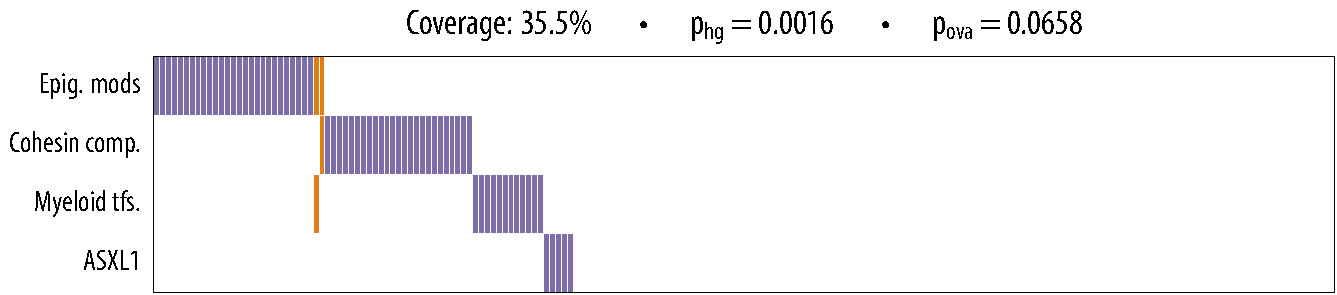
\includegraphics[width=\textwidth]{figures/genes/aml_comet1.pdf}\\[2em]
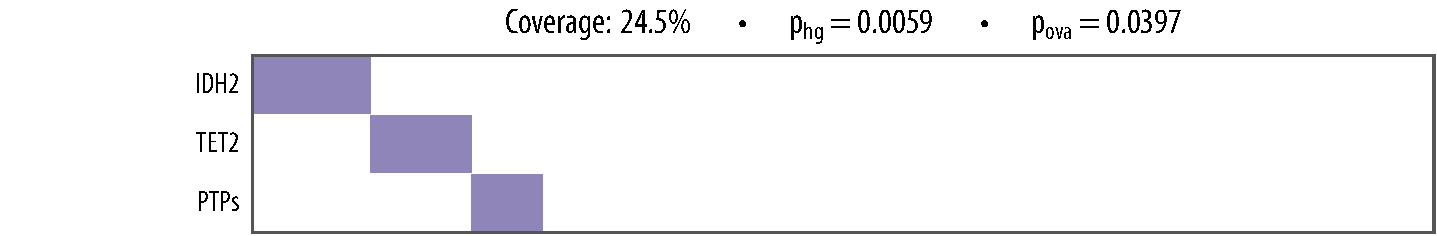
\includegraphics[width=\textwidth]{figures/genes/aml_comet2.pdf}\\[2em]
\caption{Two more groups reported by \comet{} as mutually exclusive, which our method rejects due to the high $p_{\textrm{ova}}$ values.}
\label{fig:comet_aml}
\end{figure}
\vspace{3em}
\begin{figure}[htbp]
\centering
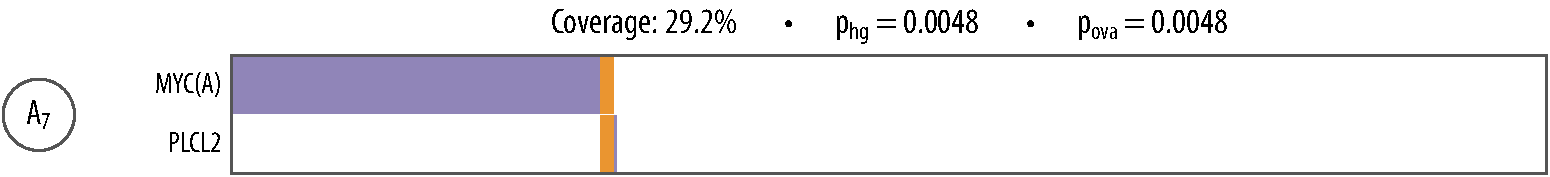
\includegraphics[width=\textwidth]{figures/genes/brca_9_a.pdf}\\[1.2em]
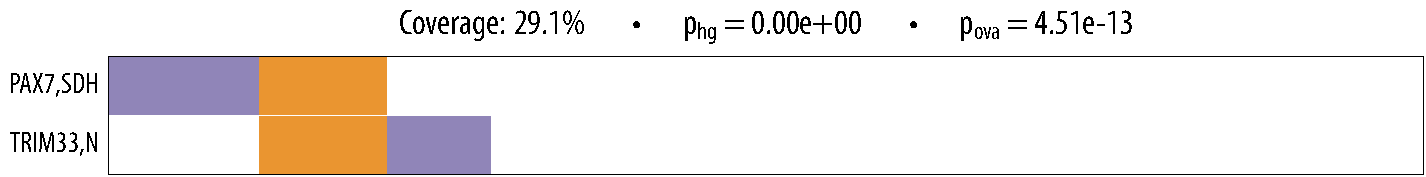
\includegraphics[width=\textwidth]{figures/genes/brca_13_a.pdf}\\[1.2em]
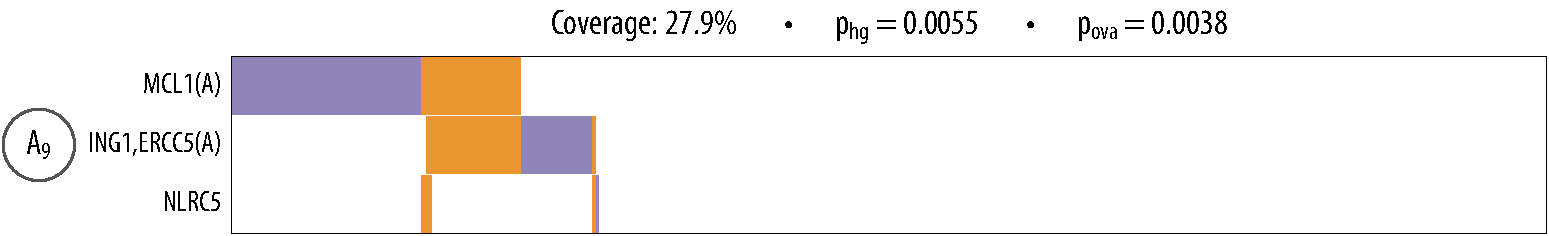
\includegraphics[width=\textwidth]{figures/genes/brca_5_a.pdf}\\[1.2em]
\caption{The next three co-occurring groups extracted from the TCGA BRCA data set.}
\label{fig:att_brca_2}
\end{figure}

\begin{figure}[htbp]
\centering
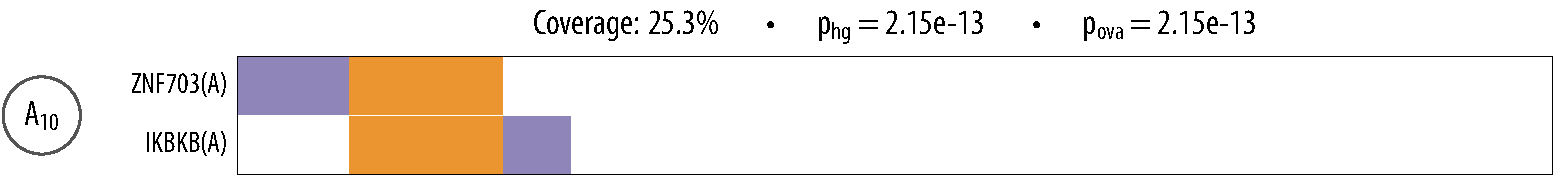
\includegraphics[width=\textwidth]{figures/genes/brca_10_a.pdf}\\[1.2em]
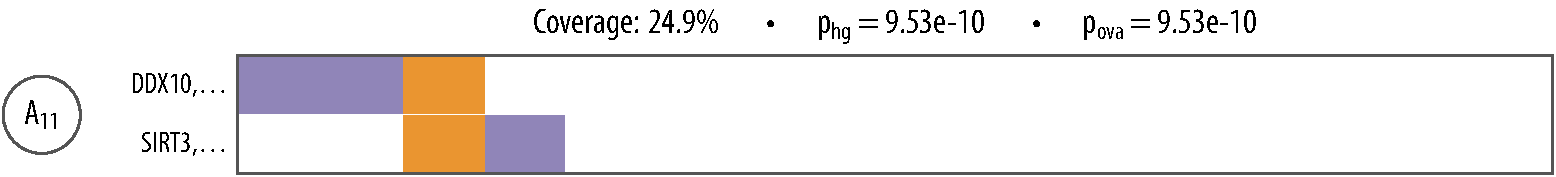
\includegraphics[width=\textwidth]{figures/genes/brca_12_a.pdf}\\[1.2em]
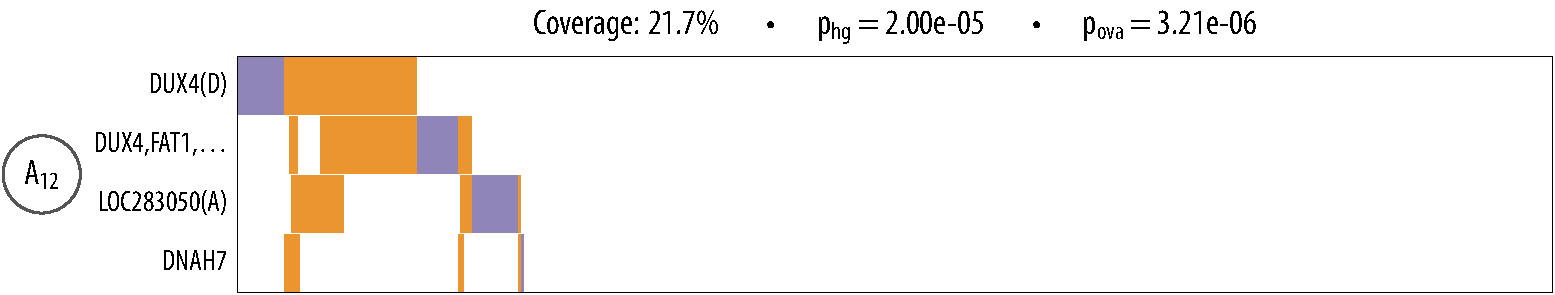
\includegraphics[width=\textwidth]{figures/genes/brca_3_a.pdf}\\[1.2em]
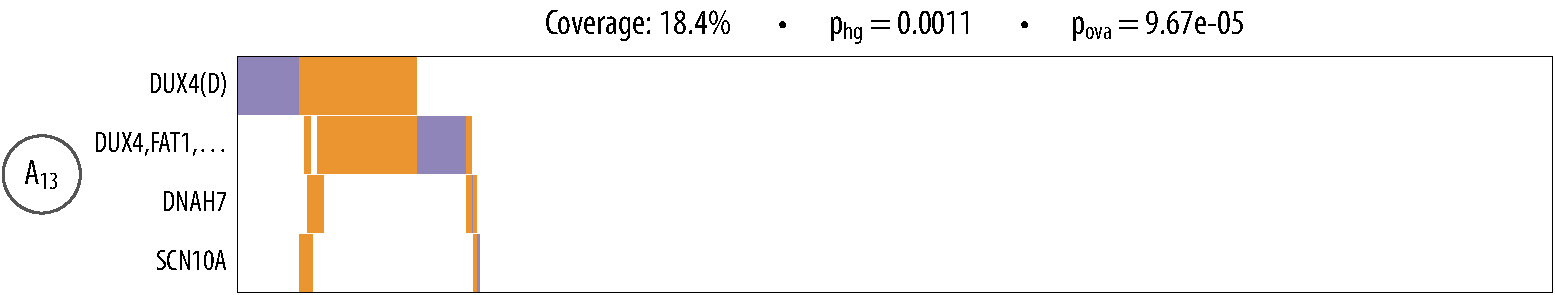
\includegraphics[width=\textwidth]{figures/genes/brca_2_a.pdf}\\[1.2em]
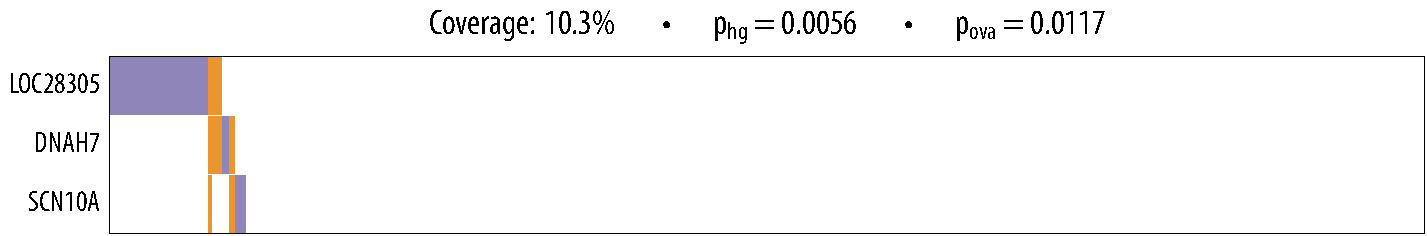
\includegraphics[width=\textwidth]{figures/genes/brca_6_a.pdf}\\[1.2em]
\caption{The rest of the co-occurring groups extracted from the TCGA BRCA data set.}
\label{fig:att_brca_3}
\end{figure}